\begin{figure}[H]
    \centering
    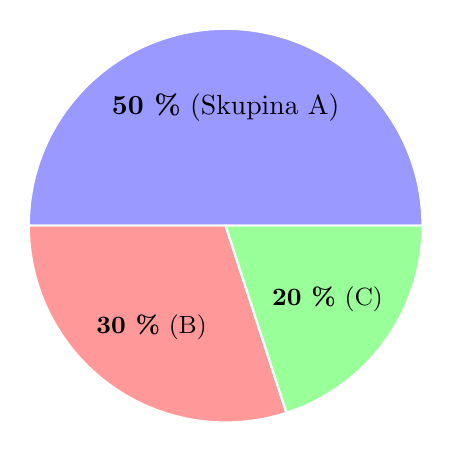
\begin{tikzpicture}
        % Kreslení kruhového grafu pomocí čistého TikZ (bez nutnosti dalších balíčků)
        % 50% = 180 stupňů, 30% = 108 stupňů, 20% = 72 stupňů
        \draw[fill=blue!40, thick, draw=white] (0,0) -- (0:2.5) arc (0:180:2.5) -- cycle;
        \node at (90:1.5) {\textbf{50 \%} (Skupina A)};
        
        \draw[fill=red!40, thick, draw=white] (0,0) -- (180:2.5) arc (180:288:2.5) -- cycle;
        \node[font=\small] at (234:1.6) {\textbf{30 \%} (B)};
        
        \draw[fill=green!40, thick, draw=white] (0,0) -- (288:2.5) arc (288:360:2.5) -- cycle;
        \node[font=\small] at (324:1.6) {\textbf{20 \%} (C)};
    \end{tikzpicture}
    \caption{Kruhový graf (Podíly z celku)}
\end{figure}